\section{Data Cleaning}

\subsection{Data Sources and Initial Loading}

The analytical base consists of eight CSV files loaded into R with \texttt{stringsAsFactors} disabled. Four contain asset price series. AAPL represents a US large-cap equity. BDO represents a Philippine banking equity. BTC represents cryptocurrency. SPY is the mandated S\&P 500 benchmark. Four contain FRED macroeconomic indicators. CPI, the Consumer Price Index, measures inflation. DGS10, the 10-Year Treasury Yield, proxies the risk-free rate. FEDFUNDS, the Federal Funds Rate, captures monetary policy stance. VIX, the CBOE Volatility Index, measures market fear. Every file was inspected for structural anomalies, missing entries, and duplicate rows before any transformation. None of these issues were found in any raw dataset, for the straightforward reason that Yahoo Finance, Investing.com, and FRED deliver clean historical records without internal gaps.

\subsection{Date Standardisation}

The eight datasets arrived in three distinct date formats. This heterogeneity is not a data quality problem. It is a routine consequence of sourcing from different providers. The Yahoo Finance exports (AAPL, BTC, SPY) used POSIXct-formatted timestamps with timezone offsets, requiring \texttt{ymd\_hms} coercion followed by Date conversion. The Investing.com export (BDO) used MM/DD/YYYY, requiring \texttt{mdy} parsing. The four FRED series used ISO 8601 YYYY-MM-DD, which R parsed natively.

BDO carried three additional idiosyncrasies. A byte-order-mark character prepended to the first column header was handled by reading the file with UTF-8-BOM encoding. The volume field used abbreviated notation (2.50M) that required a regular expression to convert suffixed values to numeric equivalents. The closing price column was labelled Price rather than Close and was remapped for internal consistency. None of these adjustments altered any observed price or return value.

Every raw dataset had zero missing values and zero duplicate rows. Yahoo Finance and Investing.com report complete historical price records. FRED reports only on scheduled release dates, so every downloaded observation is a valid reading. The cleaning burden fell entirely on format normalisation. There was nothing to impute.

\subsection{Sample Period Restriction}

All eight datasets were restricted to the analysis window from January 1, 2020 through December 31, 2025. The restriction serves two purposes. It ensures uniform temporal coverage across assets whose calendars diverge. It eliminates any need to extrapolate or impute macroeconomic readings for periods where series have no observations. The resulting counts appear in Table~\ref{tab:clean_summary}.

\subsection{Canonical Business Calendar Construction}

The central methodological decision in this section is the calendar onto which all data are aligned. The raw asset datasets have divergent temporal coverage by construction. AAPL and SPY trade on the New York Stock Exchange, contributing 1,508 trading days in the window. BDO trades on the Philippine Stock Exchange, contributing 1,468 days. BTC trades continuously, contributing 2,192 days. Aligning to any single asset's calendar would either drop legitimate trading data or inflate null rates. Neither outcome is acceptable. Table~\ref{tab:calendar_compare} evaluates four alternatives.

\begin{table}[H]
  \centering
  \caption{Comparison of Calendar Approaches for the Analytical Grid}
  \label{tab:calendar_compare}
  \begin{tabular}{l S[table-format=4.0] p{3.5cm} p{4.5cm}}
    \toprule
    Approach & {Rows} & {Reproducibility} & {Accuracy} \\
    \midrule
    NYSE-only trading days & 1508 & Requires \texttt{timeDate} package and curated NYSE holiday list & Drops BDO PSE-only trading days and all BTC weekend data \\
    PSE-only trading days & 1468 & Requires manual PSE holiday list (no standard R package) & Drops AAPL and SPY NYSE-only trading days \\
    Union (NYSE $\cup$ PSE) & {1520--1540} & Requires both exchange calendars; minimal R package support for PSE & Most precise representation of available trading days across both equity exchanges \\
    Simple Mon-Fri (chosen) & 1566 & Pure base R, deterministic, fully reproducible & Minor overcount on exchange holidays, bridged by forward-fill \\
    \bottomrule
  \end{tabular}
\end{table}

The chosen approach generates a Mon-Fri business calendar through \texttt{seq.Date()}, producing 1,566 business days with no external package dependency. Exchange-specific holidays are not excluded. They are bridged by the forward-fill procedure described in the next subsection. This regular-grid design follows Ghysels (\cite{ghysels2016}), who demonstrates that a fixed-interval observation grid avoids the mis-specification problems of state-space models built on latent process representations. Each asset series was left-joined onto this canonical calendar. BTC lost 626 weekend rows. The equity assets retained the same counts after the sample restriction, minus any holidays that fell on business days.

\subsection{Forward-Fill Methodology}

After calendar alignment, missing observations persisted for three structural reasons. Macroeconomic indicators (CPI, FEDFUNDS) release at lower frequencies than the daily calendar, producing gaps that represent genuine periods without new information. DGS10 and VIX, though business-daily, do not cover every canonical calendar date because FRED publication dates do not perfectly align with the NYSE and PSE trading calendars. Asset close prices are absent on days a given exchange was closed while the canonical calendar includes that day. None of these are data errors. They are consequences of the frequency mismatch between mixed-frequency data and the chosen daily grid.

Four approaches for handling these gaps were evaluated. Table~\ref{tab:imputation_compare} reports the trade-offs.

\begin{table}[H]
  \centering
  \caption{Comparison of Imputation Approaches for Mixed-Frequency Gaps}
  \label{tab:imputation_compare}
  \begin{tabular}{l p{2.8cm} p{2.8cm} p{2.8cm} p{2.8cm}}
    \toprule
    Criterion & Forward-fill (LOCF) & Linear Interpolation & Backward-fill & Multiple Imputation \\
    \midrule
    Look-ahead bias & None & Moderate & Severe & None if properly specified \\
    Economic basis & Markets price on last known public information & Assumes linear path between releases, unsupported for step-function data & Assumes announcement was predictable, violating rational expectations & Requires distributional assumptions about missing data mechanism \\
    Implementation complexity & Single \texttt{tidyr::fill()} call & Simple but incorrect for monthly-to-daily expansion & Simple but introduces look-ahead bias & Complex, requires model specification \\
    \bottomrule
  \end{tabular}
\end{table}

Last Observation Carried Forward was chosen because it satisfies the informational efficiency condition. Market participants in real time act only on the last publicly available observation. The theoretical justification is the efficient markets hypothesis (\cite{fama1970}). Asset prices incorporate all public information at each point. If a macro variable has not been updated, the last known value is the rational expectation. This is standard practice in mixed-frequency empirical finance, where LOCF constructs daily series from lower-frequency macro releases within the MIDAS regression framework (\cite{ghysels2004}) and in GARCH-MIDAS volatility models (\cite{conrad2020}).

The claim that linear interpolation is more accurate is incorrect for this context. CPI and FEDFUNDS are step functions by construction. They change on announcement dates and are flat between them. Interpolating between two monthly CPI values would fabricate price levels that never existed. Backward-fill would use future information to fill past dates, a clear look-ahead bias. Multiple imputation would require distributional assumptions about a missing data mechanism that does not exist: the data are not missing, they are released at a lower frequency. The choice is LOCF or nothing.

\subsubsection{Macroeconomic Series}

The four FRED series were forward-filled after the calendar join.

CPI is monthly, with 71 observations in the sample window. After forward-fill, each of the 1,566 business days carries the last reported value. This is a step function that preserves the exact information set at each date. FEDFUNDS is meeting-based, with 72 observations. The rate is constant between FOMC meetings and changes only on announcement dates. Forward-fill replicates this step-function nature precisely. DGS10 is business-daily, with 1,500 observations and approximately 66 gaps relative to the canonical calendar. VIX is business-daily, with 1,535 observations and approximately 31 gaps. Both were forward-filled.

The first business days of January 2020 precede the first CPI and FEDFUNDS observations in the sample window. To avoid nulls in this initial period, the December 2019 values for CPI and FEDFUNDS were extracted from the raw source files and seeded as the initial carry-forward. This is economically correct. The December 2019 release was the last known public information available to market participants in early January 2020.

\subsubsection{Asset Close Prices and Returns}

Asset close prices were missing on calendar days where the respective exchange was closed. Philippine holidays for BDO. US holidays for AAPL and SPY. Close prices were forward-filled via LOCF because the last traded price is the best estimate of executable value on a non-trading day, consistent with the continuity convention in calendar-effect studies (\cite{schmidbauer2018}). Daily returns on these days were set to zero. No trade occurred, so no return was generated.

\subsection{Daily Return Calculation and Recalculation}

Daily returns for all four assets use the standard discrete formulation.

\begin{equation}
\text{Daily\_Return}_t = \frac{\text{Close}_t}{\text{Close}_{t-1}} - 1
\end{equation}

For AAPL, BDO, and SPY, this was computed on each asset's original data frame before the calendar join and forward-fill, using each exchange's native trading calendar. The first observation of each asset produces a missing return by construction, which becomes zero after forward-fill.

BTC required a separate recalculation. In the original 24/7 dataset, Monday returns used (Mon Close / Sun Close) minus 1. After the calendar join removed weekend rows, Sunday's close no longer exists. The lag function would reference the wrong prior day. BTC returns were recalculated on the calendar-filtered dataset so that Monday returns reflect (Mon Close / Fri Close) minus 1. This follows the standard practice in mixed-asset studies of omitting weekend cryptocurrency data to align with equity market calendars (\cite{corbet2018}).

\subsection{Pipeline Overview}

Figure~\ref{fig:data_pipeline} presents the complete data processing pipeline as a flowchart. The pipeline proceeds through eight stages: (1) loading eight raw data files from Yahoo Finance, Investing.com, and FRED; (2) date standardisation and sample period restriction to 2020--2025; (3) construction of the canonical Mon--Fri business calendar with rejection of the 24/7 and exchange-holiday alternatives; (4) left-joining each asset series onto the calendar and recalculating BTC returns using business-day arithmetic; (5) forward-filling all four macroeconomic series (CPI, DGS10, FEDFUNDS, VIX) via LOCF with December 2019 seeding; (6) forward-filling asset Close prices and zeroing daily returns on non-trading days; (7) assembling the wide-format analytical dataset and demonstrating the four join types, followed by the SQL export pipeline (pivot to long, CPI\_YoY computation, SQLite write, CSV export); and (8) the final null-free master dataset.

\begin{figure}[htbp]
  \centering
  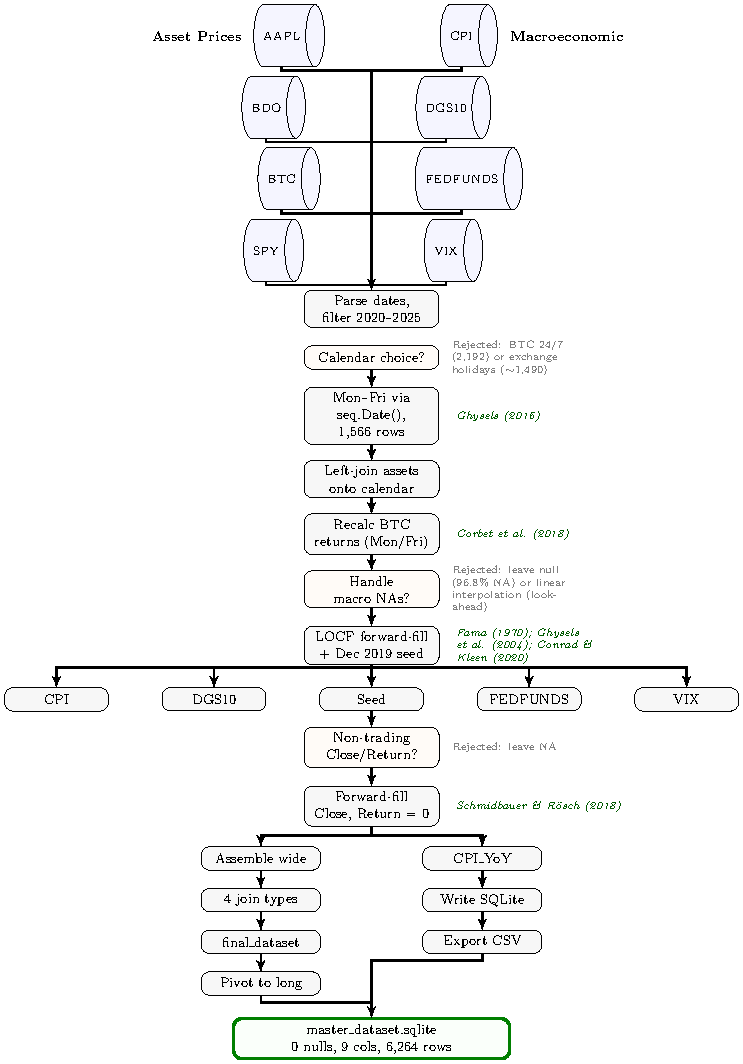
\includegraphics[width=\textwidth, height=0.75\textheight, keepaspectratio]{figures/fig_pipeline.pdf}
  \caption{Complete Data Pipeline from Raw Sources to Final Dataset. The eight layers correspond to data loading, date parsing and filtering, calendar construction, join and return recalculation, macroeconomic forward-fill, asset forward-fill, database integration and SQL export, and the final cleaned dataset. Academic citations anchoring each methodological decision are shown in green.}
  \label{fig:data_pipeline}
\end{figure}

\subsection{Observation Count Summary}

Table~\ref{tab:clean_summary} reports the observation counts at each processing stage. The After-Cleaning column reflects the sample period restriction (2020-01-01 to 2025-12-31) alone; the After-Forward-Fill column shows the expansion to the canonical \num{1566} business-day calendar.

\begin{table}[H]
  \centering
  \caption{Data Acquisition and Cleaning Summary}
  \label{tab:clean_summary}
  
\begin{tabular}{lrrr}
\toprule
Dataset & Original\_Obs & After\_Calendar\_Filter & After\_ForwardFill\\
\midrule
AAPL & 2512 & 1566 & NA\\
BDO & 2441 & 1566 & NA\\
BTC & 3652 & 1566 & NA\\
SPY & 2514 & 1566 & NA\\
CPI & 952 & 1566 & 1566\\
\addlinespace
DGS10 & 16105 & 1566 & 1566\\
FEDFUNDS & 863 & 1566 & 1566\\
VIX & 9216 & 1566 & 1566\\
Assets (wide) & NA & 1566 & NA\\
Final Dataset & NA & NA & 1566\\
\bottomrule
\end{tabular}
\end{table}
